\subsection{Biot-Savart Gesetz}
    Magnetische Wirkung eines Abschnittes eines elektrischen Leiters $\vec{dl}$ auf einen Punkt im Abstand $\left|\vec{r}\right|$   
    \mathbox{\vec{B} = \frac{\mu_0}{4 \pi} \int \frac{I \vec{dl} \times \hat{r}}{r^2}}

    \vfill \null \columnbreak

    \subsubsection{Magnetfeld gerader Draht}
        \begin{minipage}{0.39\linewidth}
            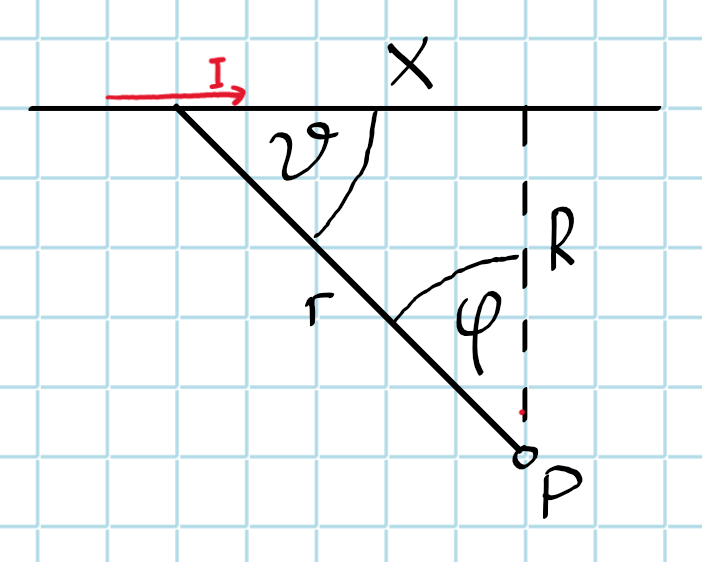
\includegraphics[width = \linewidth]{src/images/magnetfeld_draht.png}
        \end{minipage}
        \begin{minipage}{0.59\linewidth}
            \begin{empheq}[box = \fbox]{align*}
                \vec{B} &= \frac{\mu_0}{4 \pi} I \int\limits_{-\infty}^{+\infty} \frac{dx \cdot |\hat{r}| \cdot \sin{\vartheta}}{r^2}\\
                &= \frac{\mu_0}{4 \pi} I \int\limits_{-\frac{\pi}{2}}^{+\frac{\pi}{2}} \frac{\cos{\varphi}}{R} d\varphi
            \end{empheq}
        \end{minipage}
        \begin{scriptsize}
            \begin{align*}
                \sin(\vartheta) = \frac{R}{r} = \cos(\varphi) \quad &\mid \quad r = \frac{R}{\cos(\varphi)}\\
                x = R \tan(\varphi) \quad &\mid \quad dx = \frac{R}{\cos^2(\varphi)} d\varphi
            \end{align*}
        \end{scriptsize}
